\documentclass[a4paper,10pt]{article}

\usepackage[pdftex]{graphicx}
\usepackage[margin=3cm]{geometry}
\usepackage{verbatim,url}

\begin{document}

\title{
  {\normalsize
    Introduction to Algorithms, Data Structures, and Problem Solving\\
    DA4002 (HT11) Halmstad University}\\
  Assignment for Project 2: Positive-Weighted Shortest-Path (Dijkstra's Algorithm)
}
\author{
  \texttt{roland.philippsen@hh.se}
}
\maketitle



\section{Introduction}

The second project of the ITADS course focuses on more independency for the creation of an application.
It is a rather direct continuation of exercise 6.
The starting point is a skelettal implementation of a graph, some example graph definition files, and some example code fragments.
All example graphs are planar.
The task is to create an application that performs optimal path planning on directed graphs.
Each edge has a strictly positive cost, and an optimal path is one which minimizes the sum of edge costs.

Similarly to the first project, students work in teams of two, and they have to hand in \textbf{all source code} along with \textbf{a report} which documents their work and the results they obtain.
The deadline for handing in the source code and the report is \textbf{Friday, October 21, 2011, at 18h00}.

Teams who miss the deadline will receive a penalty by lowering their grade by one.
In case of exonerating circumstances, such as sickness certified by a medical doctor, a deadline extension will be granted.
Participants must notify the lecturer of such circumstances as soon as possible when they arise.



\section{Starting Point}

The source archive for the second project contains the following files:

\begin{description}

\item[Vertex.java]
  contains a bare-bones \texttt{Vertex} class, which simply contains a list of \texttt{Edge} objects that point to adjacent neighbors.
  Over the course of the project, fields need to be added here in order to support the planning algorithm.

\item[Edge.java]
  contains a bare-bones \texttt{Edge} class, which contains a reference to the \texttt{Vertex} which is at the end of the edge.
  The edge class will also need to be extended with fields, for instance the cost of traversing an edge.

\item[Graph.java]
  is a skeleton \texttt{Graph} class, which is incomplete except for the \texttt{load} method which parses adjaceny list files.
  The methods used by the \texttt{load} method have an empty body with comments describing what needs to be filled in.
  In particular, the provided \texttt{Graph} class contains no field for storing vertices.
 This is one of the first things that needs to be added in order to turn the \texttt{Graph} class into something usable.
  Several possibilities exist for storing the vertices, from bare arrays to more flexible containers~\cite{java:linked-list,java:array-list,java:hash-set,java:tree-set,java:hash-map,java:tree-map}.
  
\item[PriorityQueueExample.java]
  contains code which illustrates two different ways of using the \texttt{PriorityQueue} shipped with Java's Collection library.
  Such a priority queue~\cite{wikipedia:priority-queue} is necessary in order to implement Dijkstra's algorithm for planning the shortest path through a positive-weighted graph.
  
\item[cities.adj]
  is a text file in adjacency-list format containing a simple example graph (see figure~\ref{fig:cities}).
  Each line of the file contains two strings and a number.
  The two strings are a source and destination city, and the number is the cost of traveling from the source to the destination.
  The \texttt{cities.adj} file defines the same graph which has been used during exercise 6.
  
\item[zig-zag.adj]
  contains a graph with 510 weighted edges.
  It is based on a grid example that is illustrated in \texttt{zig-zag.png} (see also figure~\ref{fig:grid-examples}).
  This graph forms a zig-zag curve that is several vertices wide.
  Some of the edges which lie close to the border have elevated costs, but most of them have a cost of 1 or $\sqrt{2}$.
  
\item[maze.adj]
  is also based on a grid, but it is a more complex maze and contains 85226 edges (see \texttt{maze.png} and figure~\ref{fig:grid-examples}).
  This graph represents a maze, with corridors that are several vertices wide.
  Edge costs increase in the vicinity of walls.

\item[terrain.adj]
  is also based on a grid example, with 317588 edges (see \texttt{terrain.png} and figure~\ref{fig:grid-examples}).
  This graph represents an outdoors environment with a road (low edge costs), a river (very high edge costs), some grassland (low edge cost), and some forest (moderate edge costs).
  
\item[zig-zag.grid, maze.grid, and terrain.grid]
  are meant to serve as input files for one of the bonus tasks.
  They are textual representations of the images in \texttt{zig-zag.png}, \texttt{maze.png}, and \texttt{terrain.png}.
  Each line of a \texttt{.grid} file corresponds to a row of pixels in the images, but the grey scale value has been inverted and obstacles are handled specially:
  white pixels are represented with a grid value of 1, obstacles are stored as the character ``\#'', and darker tones of grey receive higher grid values.
  
\end{description}

\begin{figure}
  \centering
  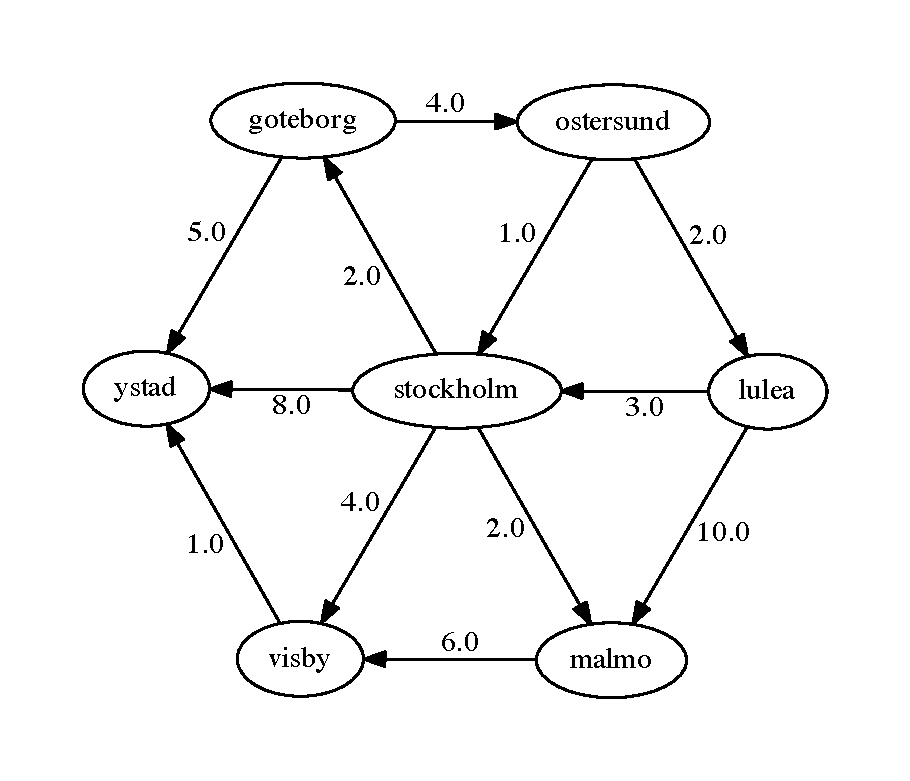
\includegraphics[width=0.6\columnwidth]{cities.pdf}
  \caption{
    Graphical representation of the graph defined in the \texttt{cities.adj} file.
  }\label{fig:cities}
\end{figure}

\begin{figure}
  \centering
  \fbox{
\includegraphics[width=0.2\columnwidth]{zig-zag.png}}
  \hfill
  \fbox{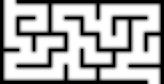
\includegraphics[width=0.35\columnwidth]{maze.png}}
  \hfill
  \fbox{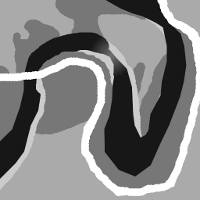
\includegraphics[width=0.35\columnwidth]{terrain.png}}
  \caption{
    Greyscale representations of the three grid-based graph examples \texttt{zig-zag.adj}, \texttt{maze.adj}, and \texttt{terrain.adj}.
    In the images, white signifies easily traversable regions (edge costs = 1), obstacles are black (non-traversable regions: no vertices or edges exist in those areas).
    Darker areas correspond to areas with higher edge costs.
    Note that the files \texttt{zig-zag.grid}, \texttt{maze.grid}, and \texttt{terrain.grid} contain the same data, but in a textual representation.
  }\label{fig:grid-examples}
\end{figure}



\section{Mandatory Tasks}

\begin{figure}
  \centering
  \fbox{
    \begin{minipage}{0.4\columnwidth}
      \footnotesize
      \verbatiminput{graph-dump-example-nocost.txt}
  \end{minipage}}
  \hfill
  \fbox{
    \begin{minipage}{0.4\columnwidth}
      \footnotesize
      \verbatiminput{graph-dump-example-cost.txt}
  \end{minipage}}
  \caption{
    Example output for printing the graph defined in \texttt{cities.adj}.
    On the left, before edge cost parsing.
    On the right, after adding edge cost support to the \texttt{Edge} and \texttt{Graph} classes.
  }\label{fig:graph-dump-example}
\end{figure}

\begin{figure}
  \centering
  \fbox{
    \begin{minipage}{\columnwidth}
      \footnotesize
      \verbatiminput{graph-dump-example-vc.txt}
  \end{minipage}}
  \caption{
    Example output for printing the graph defined in \texttt{cities.adj}.
    Here, each vertex also has a value assigned to it.
    This is indicated by the \texttt{[v: 0.0]} portion of the output.
    After running Dijkstra's algorithm, the values will be non-zero.
  }\label{fig:graph-dump-example-vc}
\end{figure}

\begin{itemize}

\item
  Extend the provided \texttt{Graph} class such that it actually creates and stores the vertices it reads from the text file.
  This implies extending the \texttt{Vertex} class such that it stores its name as well.
  Test your result by writing an application that reads \texttt{cities.adj} and prints the resulting graph on the console.
  Your output should look similar to the example given on the left in figure~\ref{fig:graph-dump-example}.
  
\item
  Extend the \texttt{Edge} class and the relevant methods in \texttt{Graph} such that edge costs get correctly parsed and stored.
  Update the test application, which should now produce output similar to the one on the right in figure~\ref{fig:graph-dump-example}.

\item
  Extend the \texttt{Vertex} class and the relevant methods in \texttt{Graph} such that you can store the cumulated path costs.
  Update the test application and its output (a more compact format is now appropriate) accoring to the example in figure~\ref{fig:graph-dump-example-vc}.

\item
  Read the information about Dijkstra's algorithm in chapter 14.3 of the course book~\cite{weiss:2005} and on Wikipedia~\cite{wikipedia:dijkstra}.
  Then implement the algorithm in a new method of the \texttt{Graph} class.
  Choose an appropriate name for this new method.
  Some \textbf{important remarks} need to be taken into account:
  \begin{itemize}
  \item
    You will need a priority queue (read the provided \texttt{PriorityQueueExample.java} file for an example).
  \item
    You will need to initialize the vertex values to ``infinity.''
    For floating-point numbers, a useful substitute for infinity is \texttt{Double.MAX\_VALUE} (which is larger than any value we would expect to encounter in a normal run of Dijkstra's algorithm).
  \item
    You will need to further extend the \texttt{Vertex} class so that it stores a backpointer to its predecessor in the optimal path.
    The Wikipedia pseudocode calls this ``\texttt{previous},'' the course book calls it ``\texttt{prev}.''
  \item
    The pseudocode given on Wikipedia relies on a priority queue which allows to re-order an item already on the queue.
    This can be avoided with the technique presented in the course book:
    simply create a new queue entry instead of re-ordering the old one.
    But this means that when you later take the old one off the queue, you have to check whether it is still relevant.
    This is explained at the beginning of page 494 in the course book.
  \end{itemize}
  
\item
  Write an application which takes three arguments:
  the name of an \texttt{.adj} file to use as graph definition, the name of the start vertex, and the name of the goal vertex.
  The application then builds the graph, applies Dijkstra's algorithm, and prints out the shortest path from start to goal.
  Note that the vertex names in the grid-based \texttt{.adj} files are based on the grid-coordinates of the cells they are based on.
  Thus, you will get a path in grid coordinates.
  Document your application, including how to run it and the paths it computes through the zig-zag (from lower-left to upper-right) and through the maze environment (from upper-left to lower-right).
  
\end{itemize}



\section{Bonus Tasks}

\begin{itemize}

\item
  Write a method which reads a \texttt{.grid} file and creates a graph from it.
  In order to convert a cell's value to vertices and edges, the following rules should be applied:
  \begin{itemize}
  \item
    If a cell is marked as an obstacle using a ``\#'' character in the \texttt{.grid} file, no vertex should be created.
    This of course also means that there will be no edges going towards or away from that cell.
  \item
    Non-obstacle cells should be connected to their four direct neighbors using edges that have a cost equal to the cell's value.
    Direct neighbors are the ones which lie to the north, east, south, or west of a cell.
  \item
    Non-obstacle cells should also be connected to their four diagonal neighbors, but with an edge cost that is $\sqrt{2}$ times the cell's value.
  \end{itemize}
  In order to preserve the grid structure in the \texttt{Graph} class, it is most appropriate to store the \texttt{Vertex} instances in a two-dimenionsional array.
  But it is also possible to keep a name-based lookup, with names that are generated from the cell indices.
  Test your implementation by loading the provided \texttt{.grid} file and comparing them to the corresponding \texttt{.adj} files.

\item
  Write a grid path planning application which takes the name of the grid file as argument, along with the coordinates of the start and goal location.
  It can also be nice to produce graphical output to show the cost map and the optimal path from start to goal.
  A simplified ``graphical'' output could be based on characters output on the console, similar to the \texttt{Mansion} class from exercise5.
  \emph{(Hint: saving the console output to a text file and viewing it in Firefox allows you to zoom out until the characters become so small that it looks almost like a greyscale image).}
  
\item
  Extend your grid path planner with heuristic search:
  implement A$^*$ search based on the description on Wikipedia~\cite{wikipedia:astar} or other resources you can find.
  Make sure you test that the paths computed using A$^*$ are the same as the ones computed with Dijkstra's algorithm.
  Compare the number of vertex expansions between A$^*$ and Dijkstra.
  
\end{itemize}



\footnotesize
\bibliographystyle{plain}
\bibliography{bibliography}

\end{document}
